
\begin{definition}
\label{definitionLineGraphe}
Soit $G = (V, E)$ un graphe non orient\'e.
\newline
Le line-graphe de $G$ est un graphe non-orient\'e $L(G) = (V',E')$ dans lequel 
$V'=E$ et 
une paire $[a,a']$ de sommets de $L(G)$ est une ar\^ete si et seulement si $a$ et $a'$ ont une extr\'emit\'e commune dans $G$.
\newline
Le graphe $G$ est appel\'e le {\em graphe racine} de $L(G)$.
\end{definition}

Si $G$ est un DAG alors  $L(G)$ est le line-graphe du graphe non-orient\'e sous-jacent \`a $G$.
\'Etant donn\'e que $G$ a $n$ sommets et $m$ arcs (sans arcs sym\'etriques), le graphe $L(G)$ a $m$ sommets et $|E'| = \sum_{i=1 }^{n} d_i(d_i -1)/2$ ar\^etes avec $d_i$ le degr\'e de chaque sommet $i$ de $G$.
\vspace{-0.3cm}

%% ---- figure GrapheRacineLineGrapheExemple
\begin{figure}[htb!]\vspace{-0.5em}
	\centering
	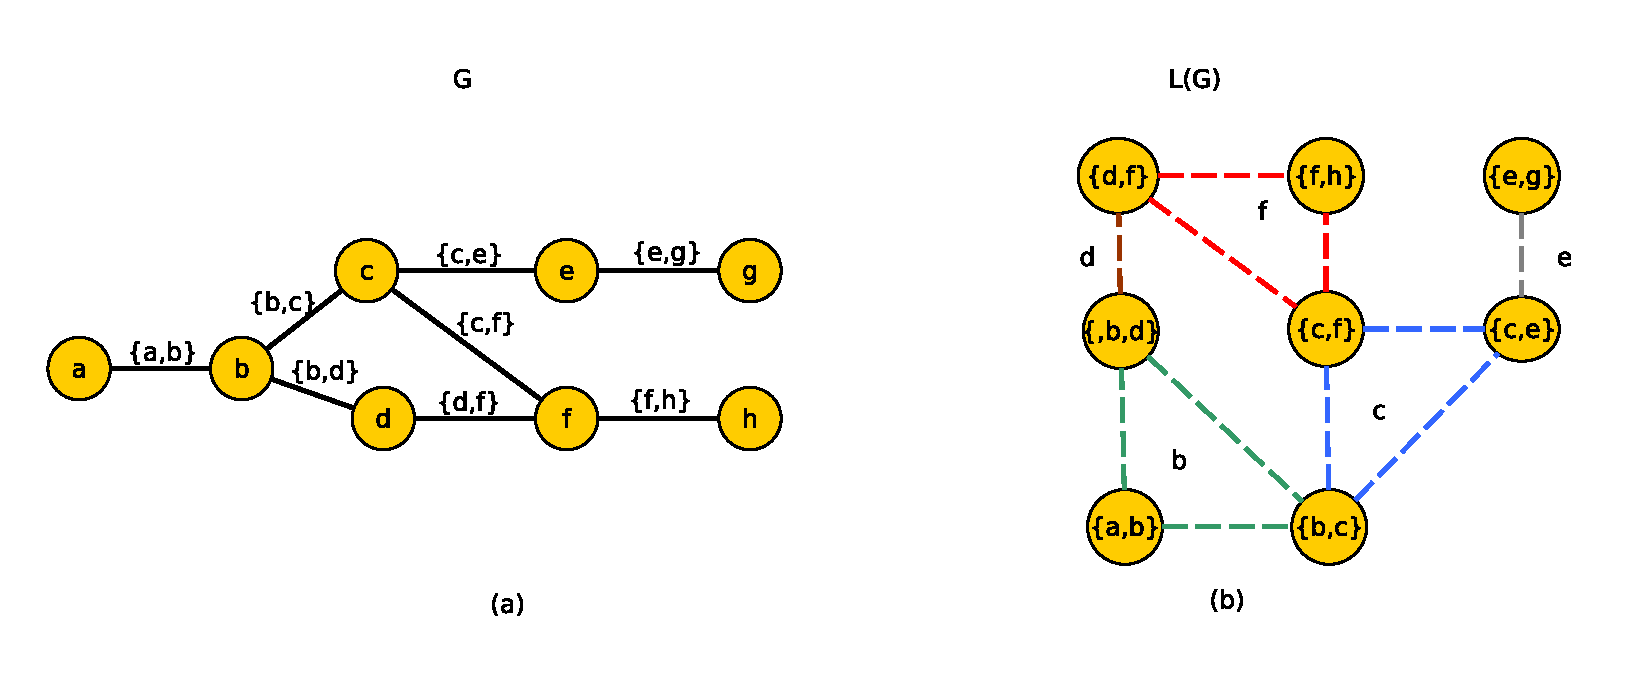
\includegraphics[scale=0.650]{grapheRacineLineGrapheExemple.eps}\vspace{-0.5em}
	\caption{ Le graphe $G$ et son line-graphe $L(G)$. 
			}\vspace{-0.5em}
	\label{grapheRacineLineGrapheExemple}
\end{figure}
%% ---- figure GrapheRacineLineGrapheExemple
\FloatBarrier
\vspace{0.3cm}

La figure \ref{grapheRacineLineGrapheExemple}(a) pr\'esente le graphe $G=(V,E)$ dans lequel l'ensemble $V$ contient $8$ sommets $V=\{a,b,c,d,e,f,g,h\}$ et l'ensemble $E$ contient $8$ ar\^etes \\ $E=\{ \{a,b\}, \{b,c\}, \{b,d\}, \{c,f\}, \{d,f\}, \{f,h\}, \{c,e\},\{e,g\} \}$. 
Chaque ar\^ete de $E$ devient un sommet de $L(G)$ dans la figure \ref{grapheRacineLineGrapheExemple}(b). Lorsque deux ar\^etes de $E$ ont une extr\'emit\'e  commune alors leurs sommets respectifs dans $L(G)$  sont adjacents.
Par exemple, dans la figure \ref{grapheRacineLineGrapheExemple}(b), les sommets $\{b,d\}$ et $\{d,f\}$ sont li\'es par une ar\^ete \`a cause du sommet $d \in V$. 
Nous construisons ainsi le graphe $L(G)$  qui contient $8$ sommets et $11$ ar\^etes.
Nous constatons qu'un sommet de $G$ correspond \`a une clique dans $L(G)$. 
En effet, les sommets de la clique $\{ \{a,b\},  \{b,c\},  \{b,d\} \}$ dans $L(G)$ concourent \`a un point $b$ qui est un sommet de $G[V]$. Le sommet  $b$ de $G$  identifie la clique $\{ \{a,b\},  \{b,c\},  \{b,d\} \}$ dans $L(G)$.
Le graphe $L(G)$ est le  line-graphe de $G$ et $G$ est le {\em graphe racine}.
\newline

La notion de {\em line-graphe} a \'et\'e introduite par {\em Whitney} \cite{whitney1932congruent} en se basant sur la notion d'isomorphisme. Il montre que  si deux line-graphes sont isomorphes et connexes alors leurs graphes racines sont aussi isomorphes \`a l'exception des graphes triangle $K_3$ et \'etoile $K_{1,3}$. 
\begin{proposition} \cite{lineGraphe}
Le graphe \'etoile $K_{1,3}$ n'est pas un {\em line-graphe}.
\end{proposition}
\begin{Proof}
{\em
Supposons que $K_{1,3}$ est le line-graphe de $H$ ($K_{1,3} = L(H)$). 
Alors $H$ est un graphe connexe de quatre ar\^etes.
Tous les graphes connexes de quatres ar\^etes sont repr\'esent\'es dans la figure  \ref{graphesRacinesDeQuatresAretes}. 
Comme $L(C_4) = C_4$  et $L(K_{1,3} + e) = K_4 + e$ (voir figure \ref{graphesRacinesDeQuatresAretes}), $L(H)$ ne peut \^etre que l'un des trois arbres $P_4$, $K_{3,2}$ et $K_{1,4}$.
Ce qui est contraire \`a notre hypoth\`ese de d\'epart ($K_{1,3} = L(H)$).}
\end{Proof}
%\newline
% ------ figure graphes Racines De Quatres Aretes
\begin{figure}[htb!]\vspace{-0.5em}
	\centering
	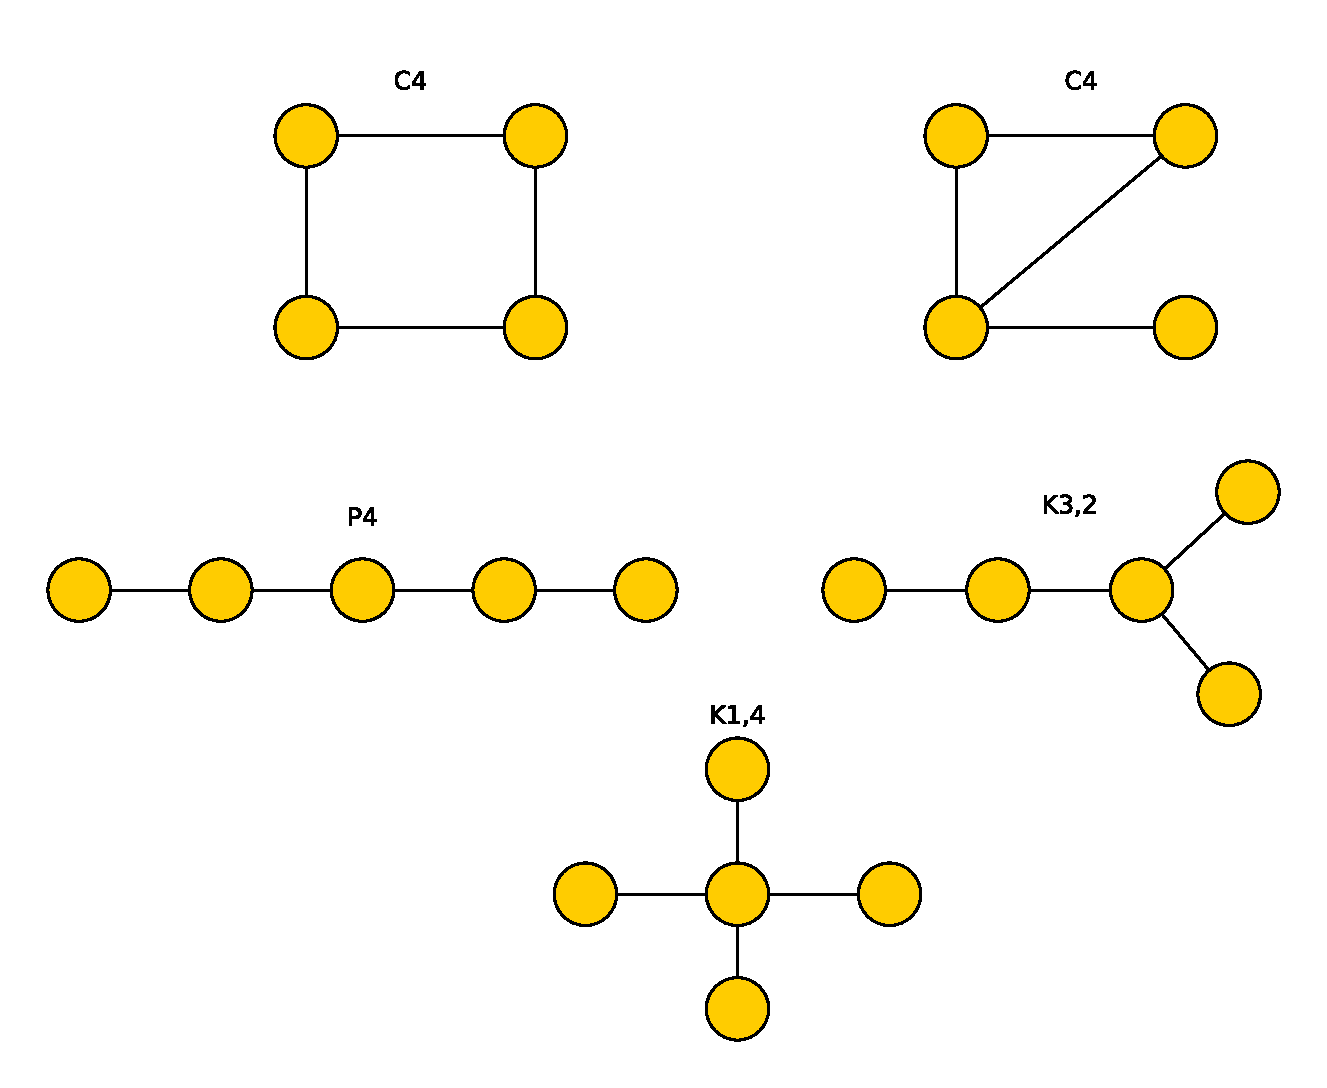
\includegraphics[scale=0.50]{graphesRacinesDeQuatresAretes.eps}\vspace{-0.5em}
	\caption{ Les graphes racines possibles de $K_{1,3}$ de quatres ar\^etes.}\vspace{-0.5em}
	\label{graphesRacinesDeQuatresAretes}
\end{figure}
% ------ figure graphes Racines De Quatres Aretes
\FloatBarrier
\vspace{0.3cm}

Le graphe \'etoile ($K_{1,3}$) a un r\^ole important dans la caract\'erisation des line-graphes.
La premi\`ere caract\'eristique provient des travaux de {\em Krausz} \cite{krausz1943demonstration} et elle est relative au partitionnement du line-graphe en sous-graphes. 
La seconde caract\'eristique, \'edit\'ee par {\em van Rooij and wilf} \cite{ROOIJetWILF1965interchange}, d\'ecrit la structure de base d'un graphe pour \^etre un line-graphe. 
Et enfin, la derni\`ere caract\'eristique pr\'esent\'ee par {\em Beineke\cite{beineke1968derived} et Hemminger} a d\'etermin\'e les neufs sous-graphes ne pouvant pas \^etre les sous-graphes induits  de line-graphes. 
\begin{theorem}\cite{lineGraphe}
%Voir theor\`eme 8.4, chapitre 8 \cite{lineGraphe}.  =====> a revoir comment je mets les references
\label{caracteristiquesLinegraphes}
Soit $H$ un graphe. Les affirmations suivantes sont \'equivalentes.
\begin{enumerate}[label = (\alph*)]
	\item $H$ est un line-graphe.
	\item Les ar\^etes de $H$ peuvent \^etre partitionn\'ees en sous-graphes complets appel\'es {\em cliques} tel qu'aucun sommet n'est contenu dans plus de deux sous-graphes. 
	\item $H$ ne contient pas $K_{1,3}$ comme sous-graphe et si deux triangles ont une ar\^ete commune alors le sous-graphe induit est $K_4$.
	\item Aucun des neufs sous-graphes de la figure \ref{neufSousGraphesInterditDesLineGraphes} ne peut \^etre un sous-graphe du line-graphe $H$.
\end{enumerate}
\end{theorem}

% ------ figure neuf Sous Graphes Interdit Des LineGraphes
\begin{figure}[htb!]\vspace{-0.5em}
	\centering
	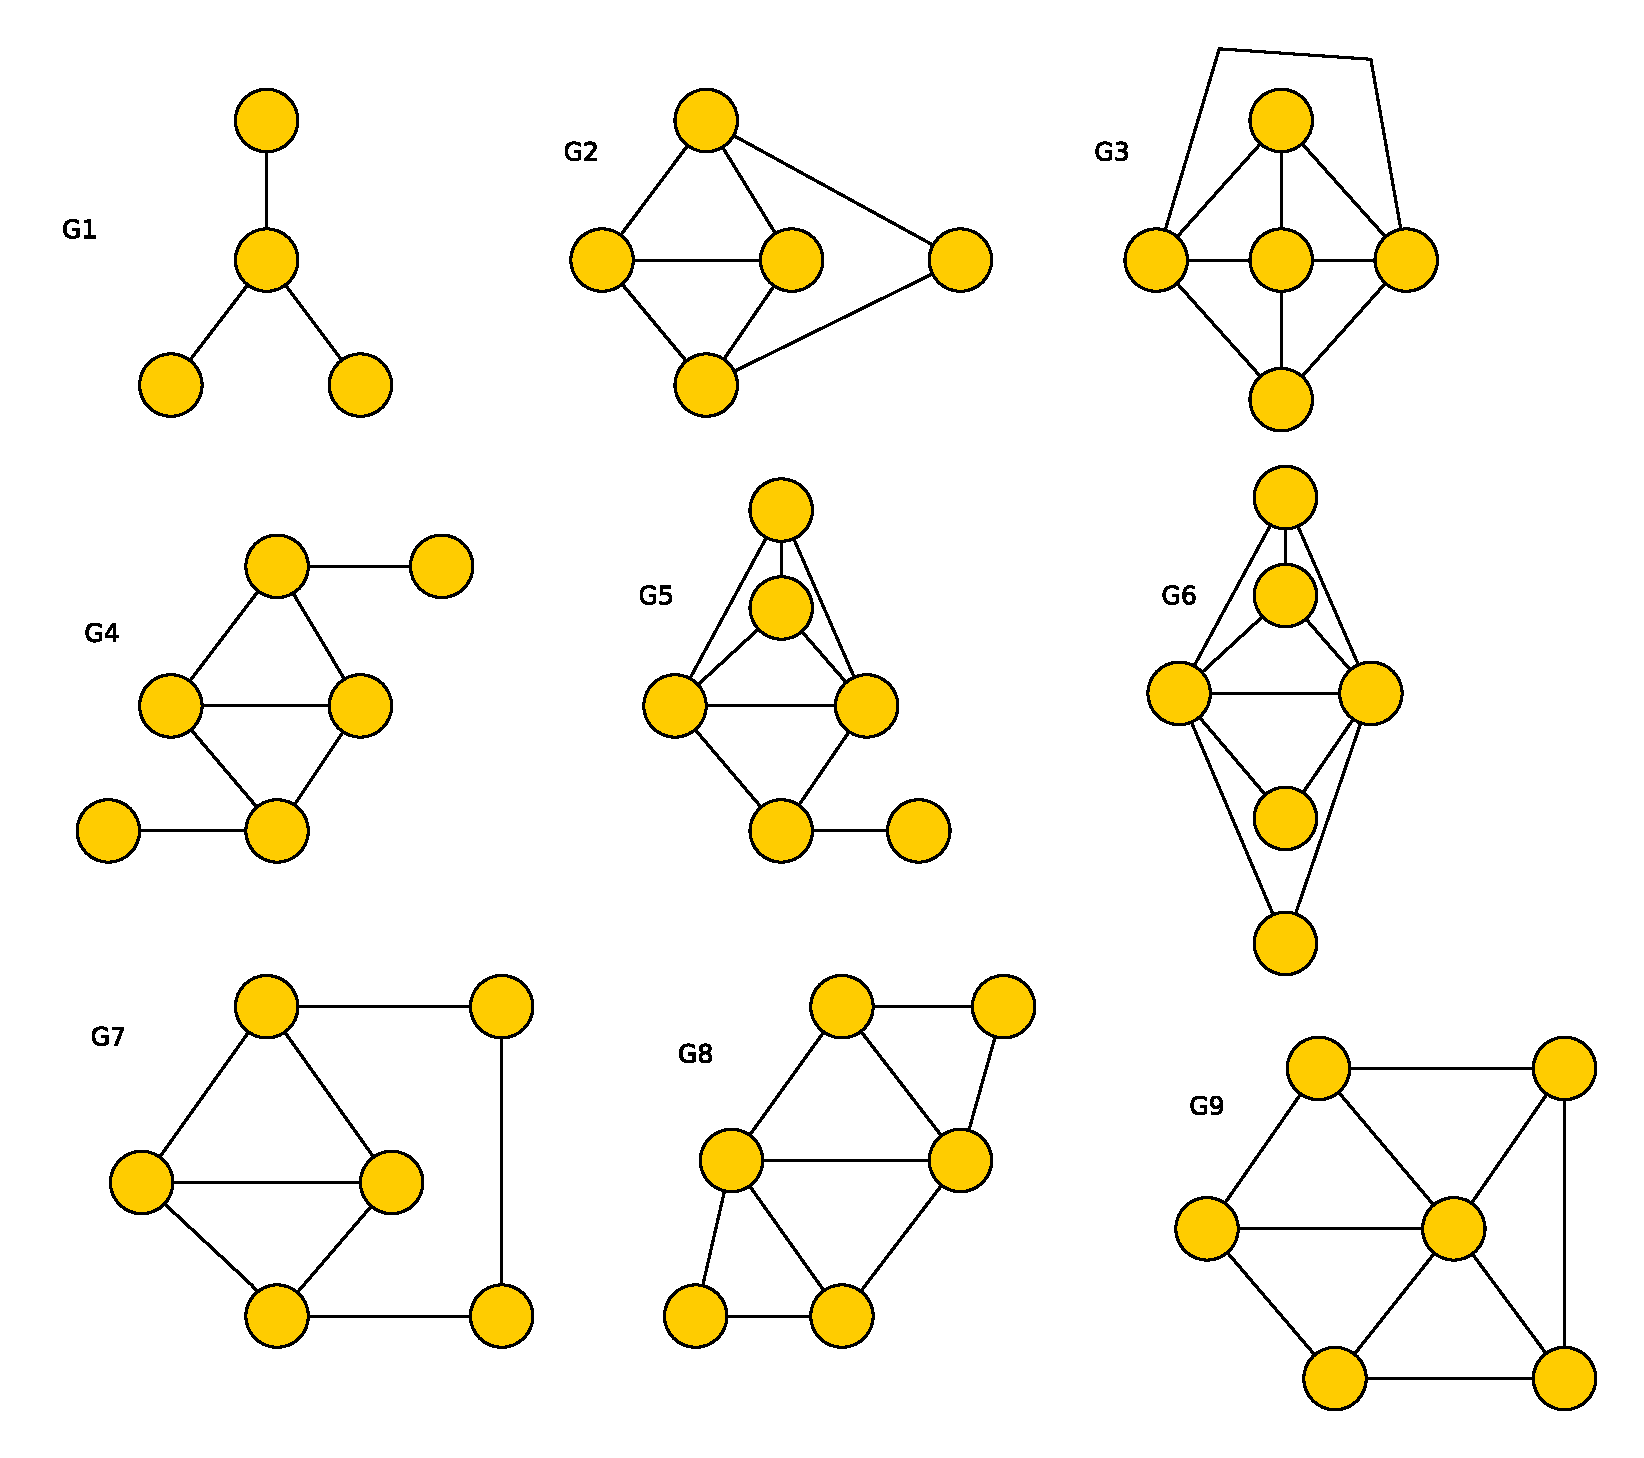
\includegraphics[scale=0.50]{neufSousGraphesInterditDesLineGraphes.eps}\vspace{-0.5em}
	\caption{ Les $9$ sous-graphes interdits dans un line-graphe. }\vspace{-0.5em}
	\label{neufSousGraphesInterditDesLineGraphes}
\end{figure}
% ------ figure neuf Sous Graphes Interdit Des LineGraphes
\FloatBarrier

{\bf Conclusion} :
soit $H$ un graphe et $G$ un graphe non-orient\'e.
Le graphe $H$ est un line-graphe de $G$ si le th\'eor\`eme \ref{caracteristiquesLinegraphes} est respect\'e.
Les graphes $H$ et $L(G)$ sont isomorphes et le graphe racine de $H$ est $L^{-1}(H)$.
Si $H$ un line-graphe d'un graphe non orient\'e $G$,
alors le graphe $H$ admet un partitionnement en cliques et chaque clique correspond \`a un sommet de $G$. L'ensemble de cliques est appel\'e une {\em couverture de corr\'elation} et est not\'e ${\cal CC}(G)$.